\documentclass[compress]{beamer}
\usepackage{ifthen,verbatim}

\newcommand{\isnote}{}
\xdefinecolor{lightyellow}{rgb}{1.,1.,0.25}
\xdefinecolor{darkblue}{rgb}{0.1,0.1,0.7}
\xdefinecolor{darkgreen}{rgb}{0.1,0.6,0.1}
%% \xdefinecolor{orange}{rgb}{0.1,0.6,0.1}
%% \xdefinecolor{purple}{rgb}{0.1,0.6,0.1}

%% Uncomment this to get annotations
%% \def\notes{\addtocounter{page}{-1}
%%            \renewcommand{\isnote}{*}
%% 	   \beamertemplateshadingbackground{lightyellow}{white}
%%            \begin{frame}
%%            \frametitle{Notes for the previous page (page \insertpagenumber)}
%%            \itemize}
%% \def\endnotes{\enditemize
%% 	      \end{frame}
%%               \beamertemplateshadingbackground{white}{white}
%%               \renewcommand{\isnote}{}}

%% Uncomment this to not get annotations
\def\notes{\comment}
\def\endnotes{\endcomment}

\setbeamertemplate{navigation symbols}{}
\setbeamertemplate{headline}{\mbox{ } \hfill
\begin{minipage}{5.5 cm}
\vspace{-0.75 cm} \small
\end{minipage} \hfill
\begin{minipage}{4.5 cm}
\vspace{-0.75 cm} \small
\begin{flushright}
\ifthenelse{\equal{\insertpagenumber}{1}}{}{Jim Pivarski \hspace{0.2 cm} \insertpagenumber\isnote/\pageref{numpages}}
\end{flushright}
\end{minipage}\mbox{\hspace{0.2 cm}}\includegraphics[height=1 cm]{../cmslogo} \hspace{0.1 cm} \includegraphics[height=1 cm]{../tamulogo} \hspace{0.01 cm} \vspace{-1.05 cm}}

\begin{document}
\begin{frame}
\vfill
\begin{center}
\textcolor{darkblue}{\Large Muon Tracking and Alignment}

\vfill
\begin{columns}
\column{0.3\linewidth}
\begin{center}
\large
\textcolor{darkblue}{Jim Pivarski}
\end{center}
\end{columns}

\begin{columns}
\column{0.3\linewidth}
\begin{center}
\scriptsize
{\it Texas A\&M University}
\end{center}
\end{columns}

\vfill
 4 August, 2009

\end{center}
\end{frame}

%% \begin{notes}
%% \item This is the annotated version of my talk.
%% \item If you want the version that I am presenting, download the one
%% labeled ``slides'' on Indico (or just ignore these yellow pages).
%% \item The annotated version is provided for extra detail and a written
%% record of comments that I intend to make orally.
%% \item Yellow notes refer to the content on the {\it previous} page.
%% \item All other slides are identical for the two versions.
%% \end{notes}

\small

\begin{frame}
\frametitle{Muon tracking}
\begin{itemize}
\item You just heard about tracking in the silicon tracker; now extend that to the muon system
\item Modular tracking environment: tracking in self-contained chambers

\begin{center}
map of muon stations (CMS quarter view)
\includegraphics[width=0.8\linewidth]{muon_system_labeled.pdf}
\end{center}
\end{itemize}
%% \hspace{-0.83 cm} \textcolor{darkblue}{\Large Outline2}
\end{frame}

\begin{frame}
\frametitle{Muon tracking}

\begin{itemize}
\item Inside of each chamber are 6--12 detector layers sensitive to
  the positions of passing muons (100--300~$\mu$m)
\item Each can measure the position and direction of local tangents to
  the muon's trajectory called \textcolor{darkgreen}{segments}
\end{itemize}

\vfill
\begin{columns}
\column{0.5\linewidth}
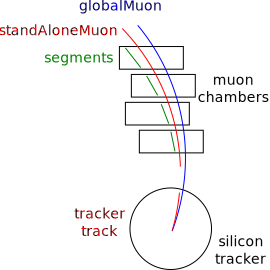
\includegraphics[width=\linewidth]{pieces.pdf}
\column{0.5\linewidth}
\begin{itemize}
\item Connect segments into a continuous track called a
  \textcolor{red}{standAloneMuon} (used especially in HLT trigger)
\item Match to closest \textcolor{red}{tracker track} to form a
  \textcolor{blue}{globalMuon}
\end{itemize}

\vspace{2 cm}
\end{columns}
\end{frame}

\begin{frame}
\frametitle{Muon tracking}

\vspace{0.5 cm}
\begin{columns}
\column{0.5\linewidth}
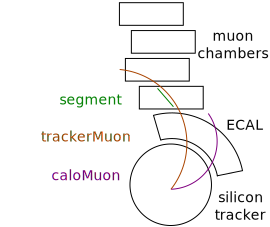
\includegraphics[width=\linewidth]{pieces2.pdf}
\column{0.5\linewidth}
Other reconstruction methods

\begin{itemize}
\item \textcolor{orange}{trackerMuon:} starting from a tracker track,
  find at least one matching \textcolor{darkgreen}{segment}
  (traditional method for experiments with smaller muon systems)
\item \textcolor{purple}{caloMuon:} match tracker track to a {\it calorimeter} shower consistent with a
  minimum-ionizing particle
\end{itemize}
\end{columns}

\vfill
\begin{itemize}
\item Purpose: high efficiency across the whole momentum range
  (low-$p_T$ tracks curl in the $\vec{B}$ field, less likely to form standAloneMuon)
\item As always, there's a trade-off between efficiency and background rejection
\item User can select from different reconstruction algorithms
\end{itemize}
\end{frame}

\begin{frame}
\frametitle{Muon tracking}

\vfill
\begin{columns}
\column{0.33\linewidth}
\textcolor{darkblue}{Efficiency} \\ {\scriptsize (high 90\%'s above 10~GeV)}

\column{0.35\linewidth}
\textcolor{darkblue}{Background rejection} \\ {\scriptsize (depends on specific analysis)}

\column{0.33\linewidth}
\textcolor{darkblue}{Resolution} \\ {\scriptsize (focus of this talk)}

\end{columns}

\begin{columns}
\column{0.33\linewidth}
\begin{itemize}
\item L1 trigger
\item HLT reco and cuts
\item offline track seeding
\item analysis cuts
\end{itemize}

\column{0.35\linewidth}
\begin{itemize}
\item $\pi \to \mu \nu$ decays in flight (so-called ``fake muons'')
\item misidentification, punch-through (actual fake muons are rare)
\end{itemize}

\column{0.33\linewidth}
\begin{itemize}
\item measuring $p_T$
\item $\vec{B}$-field outside solenoid
\item TeV muon showers
\item scattering
\item chamber alignment
\end{itemize}
\end{columns}

\vfill
\scriptsize
\begin{columns}
\column{0.5\linewidth}
\column{0.5\linewidth}
Also relevant for resolution, but not covered in this talk
\begin{itemize}\setlength{\itemsep}{-0.1 cm}
\item intrinsic hit resolution
\item calibration
\item layer alignment
\item reconstruction algorithms for TeV muon showers
\end{itemize}
\end{columns}
\end{frame}

\begin{frame}
\frametitle{Resolution}

Accuracy of reconstruction track parameters at the interaction point

\vfill
\begin{tabular}{c p{0.35\linewidth} p{0.35\linewidth}}
$\left.\begin{array}{c} d_{xy} \\ d_z \end{array}\right\}$ & point of closest approach & dominated by pixel measurements \\
$\left.\begin{array}{c} \phi \\ \lambda\mbox{, }\theta\mbox{, or }\eta \end{array}\right\}$ & direction of muon's initial momentum & dominated by strip tracker \\
$\begin{array}{c} \\ \dfrac{q}{p_T} \end{array}$ & signed curvature; magnitude of muon's initial momentum & dominated by tracker up to 200~GeV (barrel), 500~GeV (endcap); above that, both are important
\end{tabular}

\begin{itemize}
\item Direction ($\phi$, $\theta$) resolution $\sim$ (hit resolution)$/L$
\item $p_T$ resolution $\sim$ (hit resolution)$/\left(\frac{L}{2}\right)^2$
\end{itemize}


\includegraphics[width=\linewidth]{sagitta.pdf}
\end{frame}

\begin{frame}
\frametitle{Resolution}

{\scriptsize (from the TDR)}

\vfill
\includegraphics[width=0.5\linewidth]{Figure_001-005-a.pdf}
\includegraphics[width=0.5\linewidth]{Figure_001-005-b.pdf}
\end{frame}

\begin{frame}
\frametitle{Resolution}

\vspace{0.25 cm}
$Z'$ reconstructed with misaligned \textcolor{red}{tracker elements} and \textcolor{blue}{muon chambers}

\vfill
\includegraphics[width=0.95\linewidth]{misaligned_spectra.png}
\begin{itemize}
\item \textcolor{blue}{Misaligning the muon system (blue)} has a greater effect at higher momenta/$Z'$ masses
\end{itemize}
\end{frame}

\begin{frame}
\frametitle{Resolution}

\begin{itemize}
\item Further complicated by the fact that muon tracks are not helices
\end{itemize}

\includegraphics[width=\linewidth]{cms_slice.png}

\vfill
\begin{columns}
\column{0.5\linewidth}
\begin{center}
\textcolor{darkblue}{inside the solenoid}
\end{center}
\column{0.5\linewidth}
\begin{center}
\textcolor{darkblue}{outside (field is reversed)}
\end{center}
\end{columns}
\end{frame}

\begin{frame}
\frametitle{Magnetic field}

{\scriptsize (early TOSCA simulation from Magnetic Field Task Force)}

\includegraphics[width=0.9\linewidth]{muon_system_with_lines.png}

\begin{itemize}
\item Field lines try to follow iron return yoke: $\vec{B}(\vec{x}) \approx 0$ in \mbox{most chambers\hspace{-1 cm}}
\end{itemize}
\end{frame}

\begin{frame}
\frametitle{Average energy loss: $\langle dE/dx \rangle$}

\vspace{0.5 cm}
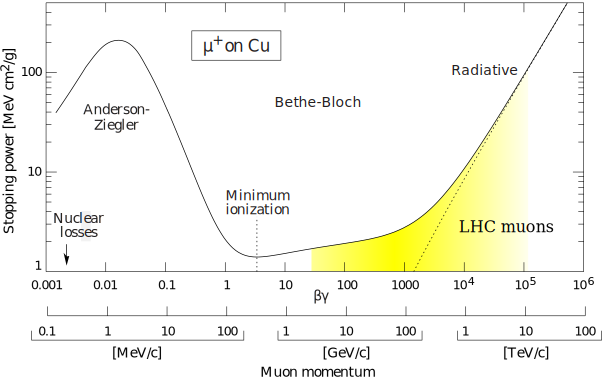
\includegraphics[width=0.95\linewidth]{pdg_muonsthroughmatter_simplified.pdf}

\begin{itemize}
\item Highest-energy muons from LHC collisions will have qualitatively different behavior in material: TeV muon showers
\end{itemize}
\end{frame}

\begin{frame}
\frametitle{TeV muon showers}

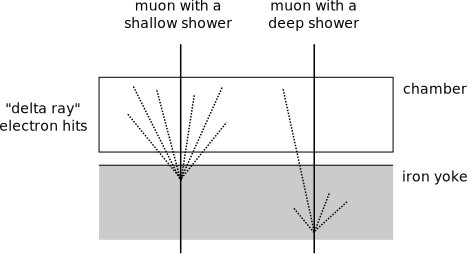
\includegraphics[width=0.65\linewidth]{showers.pdf}

\hfill 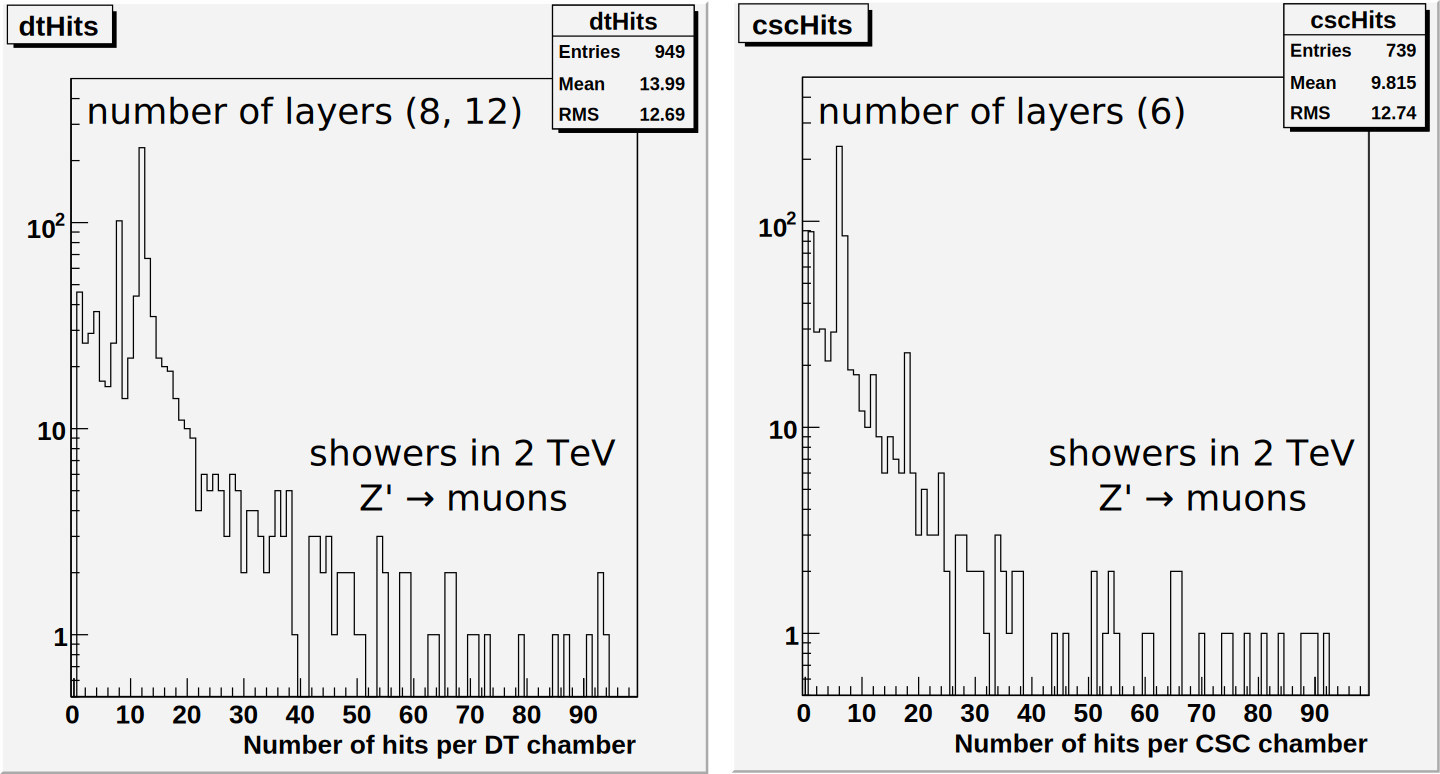
\includegraphics[width=0.75\linewidth]{hits_in_showers.pdf}
\end{frame}

\begin{frame}
\frametitle{Low-$p_T$ scattering}

\begin{itemize}
\item In the minimum-ionizing regime, track-by-track energy loss can
  be non-negligible compared to energy
\item Limit of many soft interactions (``multiple scattering'') $\to$ Gaussian
\item Single hard scattering has power-law tails
\item Real distribution is a convolution of both, highly dependent \mbox{on energy\hspace{-1 cm}}
\end{itemize}
\begin{center}
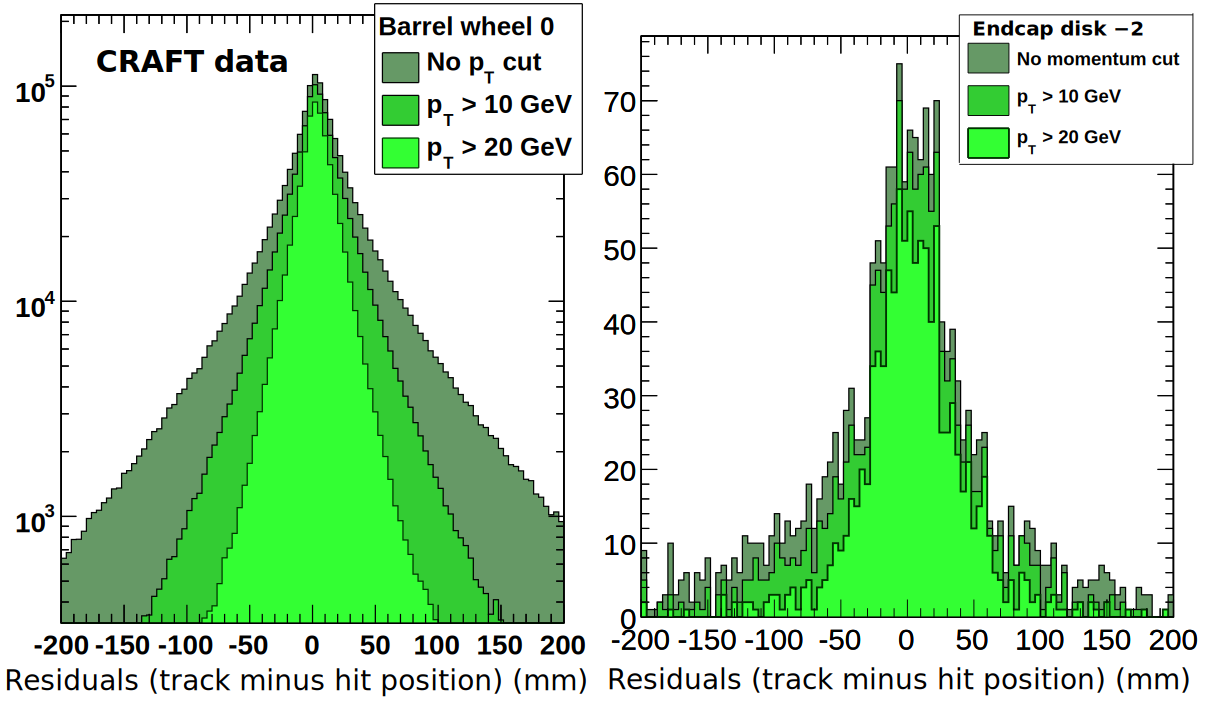
\includegraphics[width=0.85\linewidth]{residuals_with_tails.pdf}
\end{center}
\end{frame}

\begin{frame}
\frametitle{Muon alignment with tracks}

\vspace{0.5 cm}
\hfill \includegraphics[width=0.35\linewidth]{hip_explanation.pdf}

\vspace{-3.75 cm}
\begin{enumerate}
\item Select globalMuons
\item Re-fit them to the tracker only
\item Propagate to the muon system
\item Convert peak of residuals distribution \\ (track intersections minus hit positions) \\ into alignment corrections
\end{enumerate}

Matches muon chamber positions to tracks given by the tracker

\vspace{0.5 cm}
\hspace{-0.83 cm} \textcolor{darkblue}{\Large Motivation}
\begin{itemize}
\item Decouples track-fitting from alignment
\item Tracker dominates resolution for most ($p_T \ll 200$~GeV) tracks anyway
\item Peak of residuals distribution is where minimally scattered tracks agree on chamber position; highly-scattered tracks disagree in different ways (possibly asymmetric tails)
\end{itemize}
\end{frame}

\begin{frame}
\frametitle{Sample alignment fits}

\begin{itemize}
\item Model misalignment effects and propagation effects in a single ansatz, fit with Minuit
\item 4-D residuals (position and angle) $\to$ 6 rigid body \mbox{degrees of freedom\hspace{-1 cm}}
\end{itemize}

\begin{columns}
\column{0.5\linewidth}
\only<1-2>{\textcolor{darkblue}{MC before alignment}}
\only<3>{\textcolor{darkblue}{CRAFT data before alignment}}

\only<1-2>{\includegraphics[width=\linewidth]{exampleMC_wh0st1sec10_before.png}}
\only<3>{\includegraphics[width=\linewidth]{exampleData_wh0st1sec10_before.png}}

\column{0.5\linewidth}
\only<2>{\textcolor{darkblue}{MC after alignment}}
\only<3>{\textcolor{darkblue}{CRAFT data after alignment}}

\only<1>{\includegraphics[width=\linewidth]{dt_coordinates.pdf}}
\only<2>{\includegraphics[width=\linewidth]{exampleMC_wh0st1sec10_after.png}}
\only<3>{\includegraphics[width=\linewidth]{exampleData_wh0st1sec10_after.png}}
\end{columns}
\end{frame}

\begin{frame}
\frametitle{MC alignment results}

\begin{itemize}
\item MC simulation of CRAFT alignment (DT wheels $-$1, 0, $+$1)
\item Everything is the same as real-data alignment except
\begin{itemize}
\item perfect tracker alignment, magnetic field, \mbox{internal DT alignment\hspace{-1 cm}}
\end{itemize}
(to test chamber alignment procedure only)
\item Final $x$ misalignment is $\mathcal{O}($100--300~$\mu$m$)$, like hit resolution
\end{itemize}

\includegraphics[height=0.95\linewidth, angle=90]{hip_MC_simple2.pdf}
\end{frame}

\begin{frame}
\frametitle{CRAFT data alignment results}

\begin{itemize}
\item High-level test: split each cosmic ray into two LHC-like halves, fit top and bottom independently
\begin{itemize}
\item any mismatch in $1/p_T$ is purely instrumental
\item select $p_T \gtrsim 200$~GeV to emphasize contribution of the muon alignment (long lever arm for resolution of small sagitta)
\end{itemize}
\end{itemize}

\vspace{-0.5 cm}
\begin{columns}
\column{0.4\linewidth}
\begin{center}
\textcolor{darkblue}{Before muon alignment}

\includegraphics[width=\linewidth]{without_alignment.pdf}
\end{center}
\column{0.4\linewidth}
\begin{center}
\textcolor{darkblue}{After muon alignment}

\includegraphics[width=\linewidth]{with_alignment.pdf}
\end{center}

\column{0.3\linewidth}
\mbox{ }

\vspace{0.15 cm}
\scriptsize \centering \textcolor{darkblue}{Plot from Technical Design Report}

\textcolor{darkblue}{(no misalignment)}

\vspace{0.2 cm}
\includegraphics[width=\linewidth]{Figure_001-005-a_newcolors.pdf}

sigma $\sim$ 0.025 at 200~GeV for a perfect detector
\end{columns}

\vspace{-0.3 cm}
\scriptsize \hspace{3 cm} \textcolor{darkblue}{J.~Tucker}
\end{frame}

\begin{frame}
\frametitle{What about the endcaps?}

\begin{itemize}
\item Cosmic rays for alignment and diagnostics are mostly vertical:
  incomplete coverage in endcaps from cosmic rays (many chambers have zero hits)
\item No such problem with collisions muons \\ Simulated alignment using 50~pb$^{-1}$ $pp \to \mu X$, same technique:

\begin{center} \includegraphics[height=\linewidth, angle=90]{alignment_50pb-1_csconly.pdf} \end{center}

\item M.~Schmitt and J.~Pivarski are working on methods to align endcap chambers with cosmic rays
\item Beam-halo results (next page) demonstrate understanding of detector issues in real data
\end{itemize}
\end{frame}

\begin{frame}
\frametitle{Beam-halo alignment}

\vspace{0.5 cm}
\hfill \includegraphics[width=2 cm]{overlaps.png}

\vspace{-3 cm}
Using a different method:
\begin{enumerate}
\item Extrapolate segments between pairs of \\ overlapping chambers
\item Solve system of local alignment corrections
\item Compare with independent photogrammetry (PG) \\ (which has
  210~$\mu$m, 0.23~mrad resolution)
\end{enumerate}

\vfill
\begin{columns}
\column{0.37\linewidth}
\includegraphics[width=\linewidth]{data_rphi.png}
\column{0.37\linewidth}
\includegraphics[width=\linewidth]{data_phiz.png}
\column{0.26\linewidth}
9~minutes of LHC beam-halo data!
\end{columns}
\end{frame}

\begin{frame}
\frametitle{Hardware alignment}
\begin{itemize}
\item Muon system is instrumented with physical position detectors
\item Complimentary to track-based alignment
\end{itemize}

Only showing laser monitors on an endcap disk:

\vspace{0.1 cm}
\hfill \includegraphics[width=0.9\linewidth]{hardware_alignment.png}

\end{frame}

\begin{frame}
\frametitle{Hardware alignment}

\begin{itemize}
\item Bending of the endcap disks due to CMS $\vec{B}$-field
\item About 14~mm in the center (huge!), parallel to beamline ($z$)

\scriptsize (tracks are not very sensitive to CSC $z$ positions, but the displacement is large)
\end{itemize}

\includegraphics[width=\linewidth]{hardware_diskbending.png}

\vspace{-0.35 cm}
\scriptsize S.~Guragain, M.~Hohlmann
\end{frame}

\begin{frame}
\frametitle{Concluding remarks}

\begin{itemize}\setlength{\itemsep}{0.2 cm}
\item Muons are key to many signatures of new physics
\item CMS muon system has excellent signal-to-background due to its many layers in modular chambers
\item Long ``lever arm'' of muon system also helps to resolve $p_T$ of highest-momentum muons
\item Alignment is an important correction for $p_T$ resolution;
  cosmic rays and beam-halo data allow us to test our alignment
  procedures now
\item Alignment exercises revealed biases in muon tracking, other than muon misalignment (not shown here, for time)
\begin{itemize}
\item if you're looking for ways to help, I can point you to unresolved problems offline
\end{itemize}
\end{itemize}

\label{numpages}
\end{frame}

%% \section*{First section}
\begin{frame}
\begin{center}
\Huge \textcolor{blue}{Backup}
\end{center}
\end{frame}

\begin{frame}
\frametitle{Curvature resolution vs.~$p_T$}

\includegraphics[width=\linewidth]{curvature_resolution_cosmicpoint.pdf}

\begin{itemize}
\item Important caveat: MC resolution studies include the whole muon system, cosmic ray splitting (purple point) is only central DT barrel
\end{itemize}
\end{frame}

\begin{frame}
\frametitle{Mass resolution vs.~mass}

\includegraphics[width=\linewidth]{mass_resolution.pdf}

\begin{itemize}
\item Important caveat: not signed-off by $J/\psi$ and $Z$ groups
\end{itemize}
\end{frame}

\end{document}
